% Created 2015-02-08 Sun 01:39
\documentclass[11pt]{article}
\usepackage[utf8]{inputenc}
\usepackage{lmodern}
\usepackage[T1]{fontenc}
\usepackage{fixltx2e}
\usepackage{graphicx}
\usepackage{longtable}
\usepackage{float}
\usepackage{wrapfig}
\usepackage{rotating}
\usepackage[normalem]{ulem}
\usepackage{amsmath}
\usepackage{textcomp}
\usepackage{marvosym}
\usepackage{wasysym}
\usepackage{amssymb}
\usepackage{amsmath}
\usepackage[version=3]{mhchem}
\usepackage[numbers,super,sort&compress]{natbib}
\usepackage{natmove}
\usepackage{url}
\usepackage{minted}
\usepackage{underscore}
\usepackage[linktocpage,pdfstartview=FitH,colorlinks,
linkcolor=blue,anchorcolor=blue,
citecolor=blue,filecolor=blue,menucolor=blue,urlcolor=blue]{hyperref}
\usepackage{attachfile}
\usepackage[left=1in, right=1in, top=1in, bottom=1in, nohead]{geometry}
\usepackage{fancyhdr}
\usepackage{hyperref}
\usepackage{setspace}
\usepackage[labelfont=bf]{caption}
\usepackage{amsmath}
\usepackage{enumerate}
\usepackage[parfill]{parskip}
\date{Due: \textit{<2015-01-27 Tue>}}
\title{}
\begin{document}

\title{Homework 2\\Computational Chemistry\\(CBE 60553)}
\author{Prof. William F.\ Schneider}
\maketitle


\section{Lectures 1-2: Review of quantum mechanics}
\label{sec-1}

An electron is trapped in a \uline{one-dimensional} box described by the potential (recall 1 bohr = 0.529177 Å, is the atomic unit of length):

\begin{center}
\begin{equation}
    V(x)= 
\begin{cases}
    0, & -1  < x < 1  \text{ bohr} \\
    \infty, & x \leq -1 \text{ or } x \geq 1  \text{ bohr}
\end{cases}
\end{equation}
\end{center}

\begin{enumerate}[(a)]
\item Using the energy expression given in class, calculate the ground state (n=1) energy of the electron, in Hartree (the atomic unit of energy), in eV, and in kJ mol$^{\text{–1}}$.

\item We found in class that the ground-state wavefunction for this electron is $\psi_{1}(x) = cos (\pi x/2)$. Sketch this wavefunction and show that it obeys the proper boundary conditions, has zero nodes, and is normalized.

\item Suppose you approximate the true ground-state wavefunction by $\phi_{1}(x) = 1 - x^{2}$. Calculate the expectation value of the energy (in Hartree) for this approximation. How does your answer compare to the energy you calculated in (a)?

\item Can you guess an even better approximate wavefunction? Guess a candidate, evaluate the expectation value of its energy, and compare to question (c). Did you do any better than my guess?
\end{enumerate}



\subsection{Solution}
\label{sec-1-1}

\subsubsection{a)}
\label{sec-1-1-1}

We have,

$E_{n} = n^{2} \pi^{2} \hbar^{2} / 2 m_{e} L^{2}$

\begin{minted}[frame=lines,fontsize=\scriptsize,linenos]{python}
import numpy as np

# In atomic units
m = 1
hbar =1
L = 2

E_atomic = np.pi ** 2 / (2 * 2 ** 2) # hartree
E_eV = E_atomic * 27.2114
E_kJ_mol = E_atomic * 2625.4996

print 'E = {0:1.3f} hartree = {1:1.3f} eV = {2:1.3f} kJ/mol'.format(E_atomic, E_eV, E_kJ_mol)
\end{minted}

\begin{verbatim}
E = 1.234 hartree = 33.571 eV = 3239.080 kJ/mol
\end{verbatim}

\subsubsection{b)}
\label{sec-1-1-2}
The wavefunction, $\psi_{1}(x) = cos (\pi x/2)$, is plotted below. We can see that it obeys the boundary conditions. In the range, $-1 < x < 1$, $\psi$ never equals zero, so there are zero nodes. Also, $\left<\psi|\psi\right> = 1$, so the wavefunction is normalized.

\begin{minted}[frame=lines,fontsize=\scriptsize,linenos]{python}
import numpy as np
import matplotlib.pyplot as plt
from scipy.integrate import quad

x = np.linspace(-1,1)
psi = np.cos(np.pi * x / 2)

plt.plot(x,psi)
plt.xlabel('x')
plt.ylabel('$\psi$')
plt.savefig('images/1b.png')
plt.show()

# Normalizing
def integrand(x):
    return np.cos(np.pi * x / 2) ** 2

ans, err = quad(integrand, -1, 1)
print ans
\end{minted}

\begin{verbatim}
1.0
\end{verbatim}

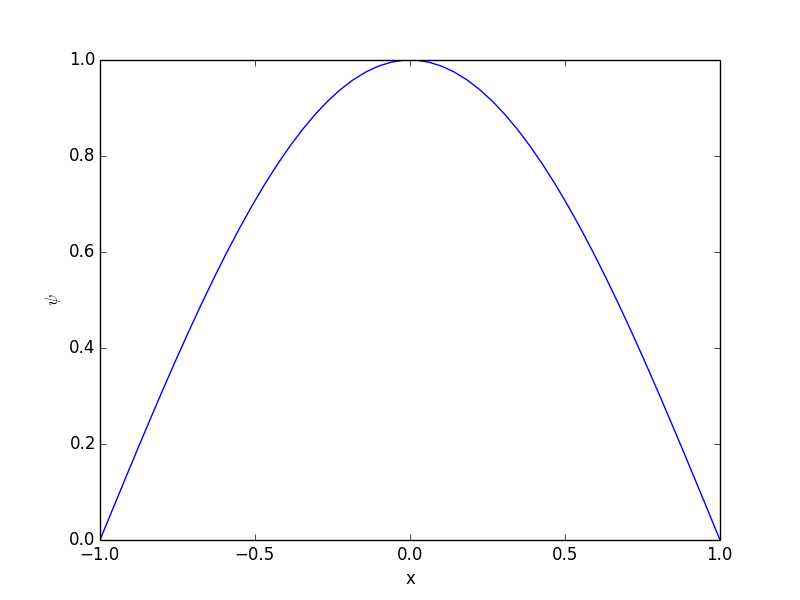
\includegraphics[width=.9\linewidth]{./images/1b.png}

\subsubsection{c)}
\label{sec-1-1-3}

First we need to normalize the wavefunction, $\phi_{1}(x) = 1 - x^{2}$. The expectation value of the energy can then be calculated using the Hamiltonian operator as $\left<E\right> = \left<\psi|H|\psi\right>$.

\begin{minted}[frame=lines,fontsize=\scriptsize,linenos]{python}
import numpy as np
from scipy.integrate import quad


# Normalizing
def integrand(x):
    return (1 - x ** 2) ** 2

c, err = quad(integrand, -1, 1)

# The wavefunction can also be written as a polynomial
# (-1*x^2 + 0*x + 1) / sqrt(c)
p = 1 / np.sqrt(c) * np.array([-1, 0, 1])

def func(x):
    return -0.5 * 1 / np.sqrt(c) * (1 - x ** 2) * np.polyder(np.polyder(p))

E, err = quad(func, -1, 1)

print 'The expectation value of the energy is {0} hartree.'.format(E)
\end{minted}

\begin{verbatim}
The expectation value of the energy is 1.25 hartree.
\end{verbatim}

We see that the energy is within 1.3 \% of part (a).

\subsubsection{d)}
\label{sec-1-1-4}


\section{Lectures 3: Many-electron atoms}
\label{sec-2}

Hartree’s father performed the first calculations on multi-electron atoms by hand. Today those same calculations (much better ones, in fact) can be done in the blink of an eye on a computer. In this problem you will use a code first developed by Herman and Skillman in the 1960’s to calculate the wavefunctions and energy of an atom using the Hartree-Fock-Slater (HFS) model, an early predecessor to DFT. The necessary software, rewritten in \texttt{C++}, is available at \verb~/afs/crc.nd.edu/users/w/wschnei1/CBE547/fda.tar.gz~.

Copy the software to your home directory, unpack (\verb~tar –xzf fda.tar.gz~), change into the directory (\verb~cd fda~) and compile the code(\verb~make fda~) to create the fda executable. Look at the \texttt{00README} file for information about the computer program and the format of the input. If you are brave, glance through the various source files (\verb~*.cxx~) to get a sense of what the code is doing. Note that the code uses atomic units, Hartree for energy and bohr for distance.

\begin{enumerate}[(a)]
\item Run the \texttt{Ar.inp} example included in the directory (\verb~fda Ar~). If all goes well, you should get an output file (\texttt{Ar.out}) and a dump file (\texttt{Ar.dmp}). Look at the \texttt{Ar.out} file to answer these questions:

\begin{itemize}
\item How many self-consistent field (SCF) iterations does the calculation take to converge?

\item What is the final calculated HFS energy of the atom?

\item What are the identities (1s, 2p, etc.) and energies of the occupied atomic orbitals?
\end{itemize}

\item The fda code solves the HFS equations on a radial grid. The \texttt{Ar.dmp} file contains the radial grid values and the total charge density in two columns of length 300, followed by an output of each orbital on the same grid. Plot out the charge density and each of the orbitals.

\item Choose one of the d block atoms. From the periodic table, figure out its electronic configuration and create an fda input file for it (follow the instructions in \texttt{00README} for how to specify the atomic number and the orbital occupancies of your atom). Run the fda calculation on your atom.

\begin{itemize}
\item What is the final calculated HFS energy of the atom? How does it compare to Ar?

\item What are the identities (1s, 2p, etc.) and energies of the occupied atomic orbitals?
\end{itemize}

\item The orbital energies are a rough approximation of the energy to remove an electron from that orbital. Use your result to estimate the first ionization energy of your atom. How does it compare with the experimental first ionization energy?

\item You can also do calculations on anions or cations. Modify the input file for your atom by removing one of the valence electrons, to make it a cation. Rerun fda on the cation. 

\begin{itemize}
\item How does the HFS energy of the cation compare to the neutral metal atom?
\item Do the energies of the orbitals go up or down from the neutral to the cation?
\item Do the electrons get closer to or further from the nucleus in the cation compared to the neutral? Use the expectation values of the distances from the nucleus (<r>) to answer the question.
\end{itemize}

\item The difference in total energy between your neutral and cation calculations is another estimate of the first ionization energy of your atom. How does this estimate compare with experiment?
\end{enumerate}



\subsection{Solution}
\label{sec-2-1}

\subsubsection{a)}
\label{sec-2-1-1}

It takes 29 iterations to converge. The final HFS energy is -526.8275 hartree. The orbital energies are tabulated below.

\begin{center}
\begin{tabular}{lr}
nl & E\\
\hline
1s & -116.9366\\
2s & -11.6037\\
2p & -9.2721\\
3s & -1.1022\\
3p & -0.5735\\
\end{tabular}
\end{center}

\subsubsection{b)}
\label{sec-2-1-2}

The Ar charge densities should be easily plottable from the code block provided in the lab.

\begin{minted}[frame=lines,fontsize=\scriptsize,linenos]{python}
import matplotlib.pyplot as plt
import numpy as np

# Lets open the file in read mode
with open('FDA/Ar.dmp', 'r') as f:

    # Reading all the lines in the file
    # Each line is stored as an element of a list
    lines = f.readlines()

    # First we read the grid points and the total charge densities
    grid_points = []
    total_charge_densities = []

    for line in lines[3:303]:

        # Each is a string with two columns
        grid_point, tot_charge_density = line.split()

        # We need to convert each line to a float add it to our lists
        grid_points.append(float(grid_point))
        total_charge_densities.append(float(tot_charge_density))

    # Alternately,
    one_s_charge_density = [float(x) for x in lines[304:604]]
    two_s_charge_density = [float(x) for x in lines[605:905]]  
    two_p_charge_density = [float(x) for x in lines[906:1206]]
    three_s_charge_density = [float(x) for x in lines[1207:1507]]
    three_p_charge_density = [float(x) for x in lines[1508:1808]]
  
plt.figure()
plt.semilogx(grid_points, total_charge_densities)
plt.xlabel('Grid Points')
plt.ylabel('Charge Density')
plt.title('Overall')
plt.savefig('images/Ar-overall-charge-density.png')

plt.figure()
plt.semilogx(grid_points, one_s_charge_density, label='1s')
plt.semilogx(grid_points, two_s_charge_density, label='2s')
plt.semilogx(grid_points, two_p_charge_density, label='2p')
plt.semilogx(grid_points, three_s_charge_density, label='3s')
plt.semilogx(grid_points, three_p_charge_density, label='3p')
plt.xlabel('Grid Points')
plt.ylabel('Charge Density')
plt.xlim(min(grid_points), max(grid_points))
plt.legend()
plt.savefig('images/Ar-orbital-charge-density.png')
plt.show()
\end{minted}

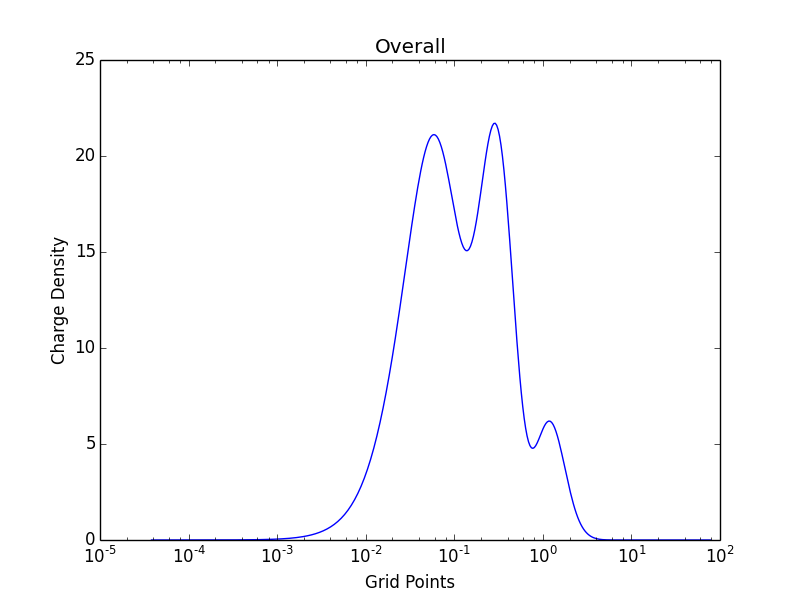
\includegraphics[width=.9\linewidth]{./images/Ar-overall-charge-density.png}

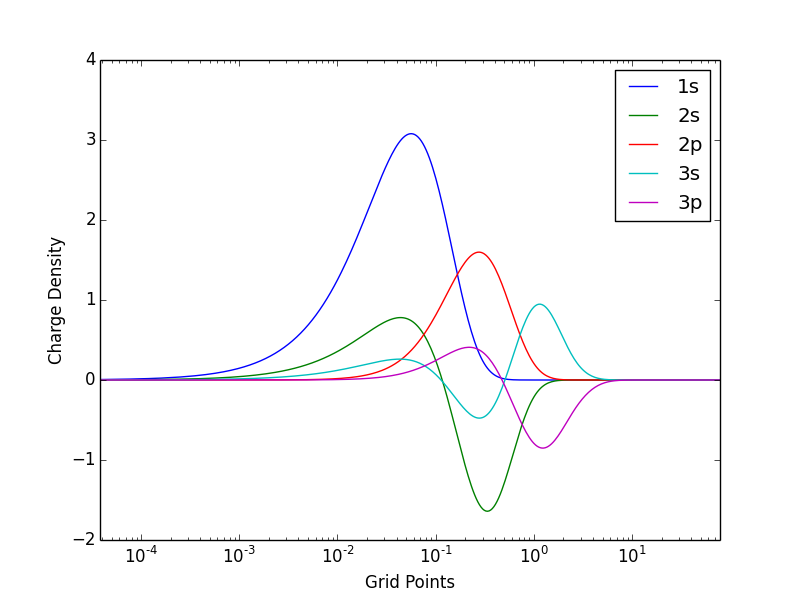
\includegraphics[width=.9\linewidth]{./images/Ar-orbital-charge-density.png}

\subsubsection{c)}
\label{sec-2-1-3}

\begin{itemize}
\item Here is an example calculation for Zn. The total energy is -1779.5562 hartree, which is about 3.5 times the energy for Ar.

\item The identities and the energies of the orbitals are below.
\end{itemize}

\begin{center}
\begin{tabular}{lrrr}
nl & occ & E & <r>\\
\hline
1s & 2.00 & -350.4349 & 0.0509\\
2s & 2.00 & -42.8635 & 0.2276\\
2p & 6.00 & -38.0715 & 0.1972\\
3s & 2.00 & -4.9959 & 0.6811\\
3p & 6.00 & -3.4181 & 0.7023\\
3d & 10.00 & -0.6922 & 0.8306\\
4s & 2.00 & -0.3265 & 2.6030\\
\end{tabular}
\end{center}


\subsubsection{d)}
\label{sec-2-1-4}

The experimental ionization energy of Zn is 906 kJ/mol. From the table we can see that our first ionization energy is 0.3265 hartree = 857.23 kJ/mol, which is about 5\% off from the experimental value. 

\subsubsection{e)}
\label{sec-2-1-5}

\begin{itemize}
\item The total energy after removing one of the cations is -1779.2279 hartree, about 0.3283 hartree more than the neutral Zn atom.

\item The orbital energies are tabulated below. All the orbital energies seem to have decreased. The 3s and 4d orbitals move closer to the nucleus.
\end{itemize}

\begin{center}
\begin{tabular}{lrrr}
nl & occ & E & <r>\\
\hline
1s & 2.00 & -350.8245 & 0.0509\\
2s & 2.00 & -43.2466 & 0.2276\\
2p & 6.00 & -38.4550 & 0.1972\\
3s & 2.00 & -5.3839 & 0.6811\\
3p & 6.00 & -3.8058 & 0.7022\\
3d & 10.00 & -1.0763 & 0.8227\\
4s & 1.00 & -0.6508 & 2.3916\\
\end{tabular}
\end{center}

\subsubsection{f)}
\label{sec-2-1-6}

The energy difference between the neutral atom and the cation is 0.3283 Hartree = 861.95 kJ/mol. This is almost the same as what we had earlier.
% Emacs 24.4.3 (Org mode 8.2.10)
\end{document}